\chapter{Propriedade da Equipartição Assintótica}

A Propriedade da Equipartição Assintótica (AEP) visa analisar o comportamento
de sequências no limite, quando estas sequências tornam-se muito grandes.  A
AEP mostra que para uma sequência longa de variáveis aleatórias independentes e
identicamente distribuídas (i.i.d.), a probabilidade de observar uma sequência
típica é aproximadamente $2^{-nH(X)}$, onde $H(X)$ é a entropia da fonte e $n$
o comprimento da sequência.

Primeiramente, vamos rever o conceito de estatística de uma amostra.
\begin{definition}[Estatístima amostral]
    Seja $x_1, x_2, \ldots, x_n$ uma sequência de comprimento $n$ de valores observados
    de uma amostra de tamanho $n$, obtidos a partir da realização de variáveis aleatórias
    $X_1, X_2, \ldots, X_n$, uma estatística de uma amostra é qualquer função calculada a partir
    de uma amostra de dados, $T(x_1, x_2, \ldots, x_n)$.
\end{definition}
Exemplos comuns incluem a média amostral
\begin{equation}
  \bar{x} = T(x_1, \ldots, x_n) = \frac{1}{n} \sum_{i=1}^n x_i ,
\end{equation}
a variância amostral
\begin{equation}
  s^2 = T(x_1, \ldots, x_n) = \frac{1}{n-1} \sum_{i=1}^n (x_i - \bar{x})^2 ,
\end{equation}
a mediana amostral, a primeira amostra $x_1$, a última amostra $x_n$,
ou até estatísticas como o máximo ou mínimo da amostra, que capturam aspectos específicos dos dados observados.
Quando avaliamos $T$ nas variáveis aleatórias $X_1, X_2, \ldots, X_n$, o resultado $T(X_1,X_2,\ldots,X_n)$
é uma variável aleatória, com sua própria distribuição.


\begin{example}[Ensaio de Bernoulli]\label{ex:ensaiobernoulliT}
  Considere o experimento de Bernoulli com $X_1, \ldots, X_n$ i.i.d., com $X_i \in \{0, 1\}$ e
  parâmetro $\theta = Pr(X_i == 1)$.

  Uma dada sequência qualquer $x_1, \ldots, x_n$ terá então probabilidade dada por
  \begin{equation}
  p(x_1,x_2,\ldots,x_n) = \prod_{i=1}^n \theta^{x_i} (1-\theta)^{1-x_i} = \theta^{\sum_i x_i} (1-\theta)^{n - \sum_i x_i}
  \end{equation}

  Considere agora a seguinte estatística
  \begin{equation}
    T(x_1,\ldots, x_n) = \sum_{i=1}^{x} x_i ,
  \end{equation}
  o somatório da amostra, no caso, a quantidade de valoes iguais a 1 que apareceu em uma realização.
  Uma vez que sabemos tal estatísticas, a probabilidade de uma sequência pode ser expressa
  sem fazer referência à $\theta$ (parâmetro que caracteriza a distribuição).
  \begin{subequations}\label{eq:TsuficienteSum}
    \begin{align}
      p(x_1,\ldots,x_n|T(x_1,\ldots,x_n),\theta) &= p(x_1,\ldots,x_n|T(x_1,\ldots,x_n)) \\
                                                &= \begin{cases}
                                                   \frac{1}{{n \choose k}} & , \sum_i x_i = k \\
                                                   0       & , \text{caso contrário}.
                                                   \end{cases}
    \end{align}
  \end{subequations}
  Em outras palavras, $X_{1:N} \independent \theta | T(X_{1:N})$. 
  Isto implica na cadeia de Markov $\theta \rightarrow T(X_{1:N}) \rightarrow X_{1:N}$.
  Aplicando a desigualdade de processamento de dados, obtemos
  \begin{equation}\label{eq:dpdtberex01}
    I(\theta;T(X_{1:N})) \geq I(\theta;X_{1:N}).
  \end{equation}
  Por outro lado, sabemos que $T(X_{1:N})$ é uma função de $X_{1:N}$.
  Desta forma, também temos a seguinte cadeia de Markov: $\theta \rightarrow X_{1:N} \rightarrow T(X_{1:N})$.
  Novamente, aplicando a desigualdade de processamento de dados, obtemos
  \begin{equation}\label{eq:dpdtberex02}
    I(\theta;X_{1:N}) \geq I(\theta;T(X_{1:N})).
  \end{equation}
  Então, para que \ref{eq:dpdtberex01} e \ref{eq:dpdtberex02} sejam satisfeitos, devemos ter
  \begin{equation}
    I(\theta;X_{1:N}) = I(\theta;T(X_{1:N})) ,
  \end{equation}
  e nenhuma informação é perdida sobre $\theta$ indo de $X_{1:N}$ para $T(X_{1:N})$.
\end{example}





\begin{definition}[Estatística Suficiente]
Uma função $T(\cdot)$ é dita ser uma estatística suficiente em relação à família
$\{f_{\theta} (x)\}$ se $X$ é independente de $\theta$ dado $T(X)$ para qualquer
distribuição em $\theta$ (i.e. $\theta \rightarrow T(X) \rightarrow X$ forma uma
cadeia de Markov). Então
\begin{equation}
I(\theta ; X) = I(\theta ; T(X)), \; \forall \theta
\end{equation}
Uma estatística suficiente preserva a informação mútua e reciprocamente
\begin{equation}
X \independent \theta | T(X) .
\end{equation}
\end{definition}

Podemos verificar que, no \Cref{ex:ensaiobernoulliT}, a estatísticas utilizada
é uma estatísticas suficiente (veja a \Cref{eq:TsuficienteSum}).


Um critério prático para identificar estatísticas suficientes é dado pelo Teorema da Fatoração de Fisher-Neyman.
\begin{theorem}
Uma estatísticas $T(X_1,\ldots,X_N)$ é suficiente para $\theta$ se, e somente se,
a função de verossimilhança da amostra pode ser escrita como:
\begin{equation}
  \mathcal{L}(\theta;x_1,\ldots,x_n) = g(T(x_1,\ldots,x_n),\theta) \cdot h(x_1,\ldots,x_n) ,
\end{equation}
onde $g$ é uma função que depende de $\theta$ e da estatística $T$, e $h$ é uma função que não depende de $\theta$.
\end{theorem}
A demonstração e mais informações sobre o tema podem ser vistos em \textcite{berger2002}.





O histograma empírico da amostra é uma estatística que descreve a distribuição de frequências relativas dos valores observados em uma amostra. 
\begin{definition}[Histograma Empírico]
  Para uma amostra $x_1,x_2,\ldots,x_n$, obtida a partir de variáveis aleatórias $X_1,X_2,\ldots,X_n$,
  com suporte finito $S_X = \{a_1,a_2,\ldots,a_D\}$, o histograma empírico pode ser definido como a
  função que associa cada símbolo $a \in S_X$ à sua frequência relativa:
  \begin{equation}
  \hat{p}_n(a) = \frac{1}{n} \sum_{i=1}^n I\{ x_i = a \} ,
  \end{equation}
  onde $I\{ x_i = a \}$ é a função indicadora
  \begin{equation}
    I\{ x_i = a \} = \begin{cases}
      1, & x = a,\\
      0, & x\neq a. 
    \end{cases}
  \end{equation}
  Desta forma, $\hat{p}_n(a)$ representa a proporção de vezes que o valor $a$ aparece na amostra.
\end{definition}
Equivalentemente, o histograma empírico pode ser representado como a enúpla que contém as frequências relativas de todos os símbolos de $S_X$.
\begin{equation}
P_{x_{1:n}} \triangleq \left( \frac{N(a_1|x_{1:n})}{n} , \frac{N(a_2|x_{1:n})}{n} , \ldots , \frac{N(a_D|x_{1:n})}{n} \right) ,
\end{equation}
onde $N(a_i|x_{1:n})$ é a contagem do número de ocorrências do símbolo $a_i$ na amostra $x_{1:n}$.
O histograma é uma estatística, já que é uma função da amostra. Podemos mostrar ainda que
o histograma empírico é uma estatísticas suficiente:
\begin{subequations}
  \begin{align}
    p(x_{1:n}|P_{x_{1:n}},\theta) &=
                \begin{cases}
                \frac{1}{{n \choose {n_1, n_2, \ldots, n_D}}} & , n_i = n P_{x_{1:n}}(a_i), \forall i \\
                0       & , \text{caso contrário}
                \end{cases} \\
                &= p(x_{1:n} \vert P_{x_{1:n}})
  \end{align}
\end{subequations}
onde temos o coeficiente multinomial\footnote{
  Teorema Multinomial
        \begin{equation}
        (x_1 + x_2 + \ldots + x_m)^n = \sum_{k_1 + k_2 + \ldots + k_m = n} {n \choose {k_1, k_2, \ldots, k_m}} \prod_{1 \leq t \leq m} x_t^{k_t}
        \end{equation}
}
${n \choose {k_1, k_2, \ldots, k_m}} = \frac{n!}{k_1! k_2! \ldots k_m!}$.
Podemos observar que $p(x_{1:n}|P_{x_{1:n}},\theta) = p(x_{1:n}|P_{x_{1:n}})$, ou seja,
é independente de $\theta$.
Então $X_{1:n} \independent \theta \vert P_{x_{1:n}}$, então $P_{x_{1:n}}$ é uma estatística suficiente.






\section{Codificação}

O codificador é responsável por associar cada sequência $x_1,x_2,\ldots,x_n$
produzida pela fonte, ou seja, realizações de variáveis aleatórias $X_1,X_2,\ldots,X_n$,
a uma sequência de bits de comprimento variável ou fixo, de modo que a sequência original 
possa ser recuperada perfeitamente por um decodificador. Para simplificar, vamos
supor que as mensagens codificadas possuem, todas elas, um mesmo comprimento $m$.
O alfabeto da fonte é $\mathcal{X} = \{a_1, a_2, \ldots, a_K\}$, possuindo assim 
cardinalidade $K = \vert \mathcal{X} \vert$. O alfabeto
de saída do codificador é $\mathcal{Y} = \{0,1\}$, ou seja, codificação binária ($\vert \mathcal{Y} \vert = 2$).
A \Cref{fig:blockcoding} representa este esquema de codificação.

\begin{figure}%
  \centering
  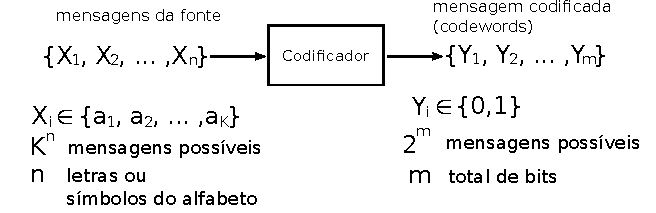
\includegraphics[width=0.8\linewidth]{figures/blockcoding.pdf}
  \caption{Esquemático de um codificador.}
  \label{fig:blockcoding}
\end{figure}

Para que seja possível termos uma palavra de código para cada mensagem possível,
devemos satisfazer a seguinte condição:
\begin{equation}
  2^m \geq K^n ,
\end{equation}
ou seja,
\begin{equation}
  m \geq (\log K) n
\end{equation}

A taxa de codificação mede a eficiência de um esquema de codificação 
ao representar uma sequência de símbolos em forma binária. 
\begin{definition}[Taxa de Codificação]
  Para uma sequência de entrada de comprimento $n$, $X_1,X_2,\ldots,X_n$,
  codificada em uma mensagem binária de comprimento $m$, $Y_1,Y_2,\ldots,Y_m$,
  a taxa de codificação é definida como
  \begin{equation}
    R = \frac{m}{n} .
  \end{equation}
  $R$ representa então o número de bits por símbolo utilizados na tarefa de codificação.
\end{definition}



Considerando que a fonte produz uma sequência de símbolos i.i.d., a probabilidade de uma
sequência qualquer de comprimento $n$ pode ser expressa por
\begin{equation}
p(X_1 = x_1, X_2 = x_2, \ldots, X_n = x_n) = \prod_{i=1}^{n} p(X_i = x_i)
\end{equation}
A informação sobre um evento é dada por $-\log p(x) = I(x)$, então a informação
associada à mensagem $x_1,x_2,\ldots,x_n$ é 
\begin{subequations}
  \begin{align}
    I(x_1,x_2,\ldots,x_n) &= - \log p(x_1, x_2, \ldots, x_n) = - \log \prod_{i=1}^n p(x_i) \\
                          &= \sum_{i=1}^n - \log p(x_i) = \sum_{i=1}^n I(x_i),
  \end{align}
\end{subequations}
onde notamos que eventos independentes são aditivos em relação a esta função de informação.
Observe que $E I(X) = H(X)$.
A lei fraca dos grandes números\footnote{
Lei dos Grandes Números: 
Se um evento de probabilidade $p$ é observado repetidamente em ocasiões independentes,
a proporção da frequência observada deste evento em relação ao total número de repetições
converge em direção a $p$ à medida que o número de repetições se torna arbitrariamente grande.

Sejam $X_1, X_2, \ldots, X_n$ v.a.s i.i.d. com $\E X_i = \mu$ e $\Var X_i = \sigma^2 < \infty$, para $i=1,\ldots,n$.
Seja a média definida por $\overline{X_n} = \frac{1}{n} \sum_{i=1}^{n} X_i$, então, para $\varepsilon > 0$,
a \emph{Lei Fraca dos Grandes Números} diz que $\overline{X_n}$ converge em probabilidade para $\mu$, ou seja,
\begin{equation}
\lim_{n \rightarrow \infty} P \left( \vert \overline{X_n} - \mu \vert < \varepsilon  \right) = 1 .
\end{equation}
}
diz que $\frac{1}{n} S_n \xrightarrow{p} \mu$, onde $S_n$ é a soma
de v.a.s i.i.d. com média $\mu = \E X_i$. Temos que $I(X_i)$ também é uma v.a. com média $H(X)$.
Obteremos assim
\begin{equation}
  \frac{1}{n} \sum_{i=1}^n I(X_i) \xrightarrow[n \rightarrow \infty]{p} H(X) .
\end{equation}
Quando $n$ é grande suficiente, podemos escrever
\begin{subequations}
  \begin{align}
     \frac{1}{n} \sum_{i=1}^n I(x_i)        &\approx H(X) , \forall i, x_i \sim p(x) \\
     - \frac{1}{n} \sum_{i=1}^n \log p(x_i) &\approx H(X) \\
     - \log \prod_{i=1}^n p(x_i)            &\approx n H(X) \\
     - \log p(x_1,x_2,\ldots,x_n)           &\approx n H(X) \\
     p(x_1,x_2,\ldots,x_n)                  &\approx 2^{-nH(X)} .
  \end{align}
\end{subequations}
Esta probabilidade não depende da sequência em si. Depende apenas do comprimento $n$ e
da entropia da fonte.
Quando $n$ fica grande, podemos dizer que todas as sequências terão a mesma probabilidade: $2^{-nH}$.
Estas sequências que possuem esta probabilidade (praticamente todas as sequências) são
chamadas de \emph{sequências típicas}, e são representadas pela conjunto $A_\epsilon^{(n)}$.

Se todas as sequência de comprimento $n$ possuem aproximadamente a mesma probabilidade $2^{-nH(X)}$,
então existe no máximo $2^{nH}$ sequências de comprimento $n$. Pode ser que $2^{nH} \ll K^n$,
ou seja, o conjunto das sequências típicas é muito menor do que o conjunto de todas as sequências
possíveis de comprimento $n$. Isto implica que, efetivamente, poderemos nos preocupar apenas
com a codificação do conjunto menor, o conjunto das sequências que efetivamente ocorrem, as sequências
típicas. Desta forma, para representar (ou codificar) as sequencias típicas, precisaremos de
$nH(X)$ bits. Teremos então
\begin{equation}
m = nH(X)
\end{equation}
no modelo do codificador. Então a taxa será $H(X)$.


\begin{theorem}[Propriedade da Equipartição Assintótica]\label{thm-prop-eqp-ass}
  Se $X_1, X_2, \ldots, X_n$ são i.i.d. e $X_i \sim p(x)$ para todo $i$, então
  \begin{equation}\label{eq-pX1X2Xn-H}
  -\frac{1}{n} \log p(X_1, X_2, \ldots, X_n) \xrightarrow{p} H(X)
  \end{equation}
\end{theorem}
\begin{proof}
  \begin{subequations}
  \begin{align}
  -\frac{1}{n} \log p(X_1, X_2, \ldots, X_n) &= - \frac{1}{n} \log \prod_{i=1}^n p(X_i) \\
                                             &= - \frac{1}{n} \sum_i \log p(X_i) \xrightarrow{p} \E \log p(X) \label{eq:dempealfgn}\\
                                             &= H(X)
  \end{align}
  \end{subequations}
  onde utilizamos a lei fraca dos números grandes em \ref{eq:dempealfgn}.
  \end{proof}


\begin{definition}[Conjunto Típico]
  Um conjunto típico $A_\epsilon^{(n)}$ em relação a $p(x)$ é o conjunto de sequências
  $(x_1,x_2,\ldots,x_n) \in \mathcal{X}^n$ com propriedade
  \begin{equation}
  2^{-n(H(X)+\epsilon)} \leq p(x_1, x_2, \ldots, x_n) \leq 2^{-n(H(X)-\epsilon)}
  \end{equation}
  De forma equivalente, podemos escrever
  \begin{equation}
  A_\epsilon^{(n)} = \left\{ (x_1, x_2, \ldots, x_n) : \vert - \frac{1}{n} \log p(x_1, \ldots, x_n) - H \vert < \epsilon \right\}
  \end{equation}
\end{definition}



\begin{theorem}[Propriedades do Conjunto Típico $A_\epsilon^{(n)}$]\label{thm:propconjtip}
\ \\ 
\begin{enumerate}
\item\label{prop1conjtip} Se $(x_1, x_2, \ldots, x_n) \in A_\epsilon^{(n)}$, então
      \begin{equation}
      H(X) - \epsilon \leq - \frac{1}{n} \log p(x_1, x_2, \ldots, x_n) \leq H(X) + \epsilon
      \end{equation}
\item\label{prop2conjtip} $p(A_\epsilon^{(n)}) = p\left( \left\{ x: x \in A_\epsilon^{(n)} \right\} \right) > 1 - \epsilon$ para $n$ grande suficiente, para todo $\epsilon > 0$.
\item\label{prop3conjtip} Limite superior: $\vert A_\epsilon^{(n)} \vert \leq 2^{n(H(X)+\epsilon)}$, onde $\vert A_\epsilon^{(n)} \vert$ é o número de elementos no conjunto $A_\epsilon^{(n)}$.
\item\label{prop4conjtip} Limite inferior: $\vert A_\epsilon^{(n)} \vert \geq (1-\epsilon) 2^{n(H(X) - \epsilon)}$ para $n$ grande suficiente.
\end{enumerate}
\end{theorem}

\begin{proof}
\ \\
\begin{enumerate}
  \item O primeiro apenas é uma reformulação da definição de AEP.
  \item Vamos utilizar a definição expandida de convergência em probabilidade,
          dada na equação \ref{eq-pX1X2Xn-H}.
          \begin{equation}
          p(A_\epsilon^{(n)}) = p\left( \vert - \frac{1}{n} \sum_i \log p(x_i) - H \vert < \epsilon \right) > 1 - \delta
          \end{equation}
          para $n$ grande suficiente.
          Podemos escolher qualquer $\delta$, escolhemos então $\delta = \epsilon$, resultando em
          \begin{equation}
          p(A_\epsilon^{(n)}) > 1 - \epsilon, \quad \text{ para } n \text{ grande suficiente } \forall \epsilon
          \end{equation}
  \item Limite superior de $A_\epsilon^{(n)}$
    \begin{subequations}
      \begin{align}
        1 &= \sum_x p(x) \geq \sum_{x \in A_\epsilon^{(n)}} p(x) \geq \sum_{x \in A_\epsilon^{(n)}} 2^{-n(H(X)+\epsilon)} \\
          &= \vert A_\epsilon^{(n)} \vert 2^{-n(H(X)+\epsilon)}
      \end{align}
    \end{subequations}
  Resultando em $\vert A_\epsilon^{(n)} \vert \leq 2^{n(H+\epsilon)}$.
  \item Limite inferior do tamanho de $A_\epsilon^{(n)}$. Para $n$ grande suficiente
    \begin{subequations}
        \begin{align}
        1 - \epsilon &< p(A_\epsilon^{(n)}) \leq \sum_{x \in A_\epsilon^{(n)}} 2^{-n(H(X)-\epsilon)} \\
                     &= 2^{-n(H(X)-\epsilon)} \vert A_\epsilon^{(n)} \vert
        \end{align}
    \end{subequations}
    resultando em $\vert A_\epsilon^{(n)} \vert \geq (1-\epsilon) 2^{n(H(X)-\epsilon)}$.
\end{enumerate}
\end{proof}

A AEP e o tamanho do conjunto típico têm implicações diretas na codificação de
sequências, como no exemplo de imagens digitais. Considere uma imagem full HD
de $1080 \times 720$ pixels, com 16 milhões de cores (24 bits por pixel, ou
seja, $2^{24}$ cores possíveis). O número total de pixels é $1080 \times
720 = 777.600$, e cada pixel é representado por 24 bits, totalizando 
$K = 1080 \times 720 \times 24 = 18.662.400 \approx 10^7$ bits por imagem. O
número total de imagens possíveis é $2^K = 2^{18.662.400} \approx 10^{5.617 \times 10^6}$, 
um valor extremamente grande, muito maior que o número de
átomos no universo observável ($\approx 10^{81}$). Pela AEP, se os pixels
fossem i.i.d. com entropia $H(X)$ (em bits por pixel), o número de imagens
típicas seria aproximadamente $2^{nH(X)}$, onde $n = 777.600$. Mesmo
que $H(X)$ fosse pequeno (por exemplo, 1 bit por pixel devido a
redundâncias), o número de imagens típicas seria $2^{777.600} \approx 10^{234.000}$, 
ainda muito maior que $10^{81}$. Isso ilustra que, embora
o número de imagens típicas seja uma fração minúscula do total, ele ainda é
astronomicamente grande, destacando a necessidade de codificação eficiente para
lidar com sequências típicas, que dominam a probabilidade.

Considere agora as chaves privadas de Bitcoin. Uma
chave privada de Bitcoin é um número de 256 bits, gerado aleatoriamente, o que
significa que o número total de chaves possíveis é $2^{256} \approx 1,1579 \times 10^{77}$. 
Esse valor é menor que o número de átomos no universo observável, mas ainda é astronomicamente grande. 
Pela AEP, se os bits da chave fossem gerados de forma i.i.d. com entropia $H(X)$
(em bits por bit), o número de chaves típicas seria aproximadamente $2^{nH(X)}$, 
onde $n = 256$. No caso ideal, em que os bits são uniformes
($H(X) = 1$ bit por bit), o número de chaves típicas é $2^{256 \cdot 1} = 2^{256}$,
ou seja, todas as chaves são típicas. No entanto, se houvesse algum
viés na geração das chaves, por exemplo, $H(X) = 0,9$ bits por bit, o
número de chaves típicas seria $2^{256 \cdot 0,9} = 2^{230,4} \approx 10^{69,3}$, 
ainda um número enorme, mas uma fração do total. Isso ilustra a
importância de maximizar a entropia na geração de chaves para garantir que o
espaço de chaves típicas seja o maior possível, minimizando a probabilidade de
colisões.

\begin{marginfigure}%
  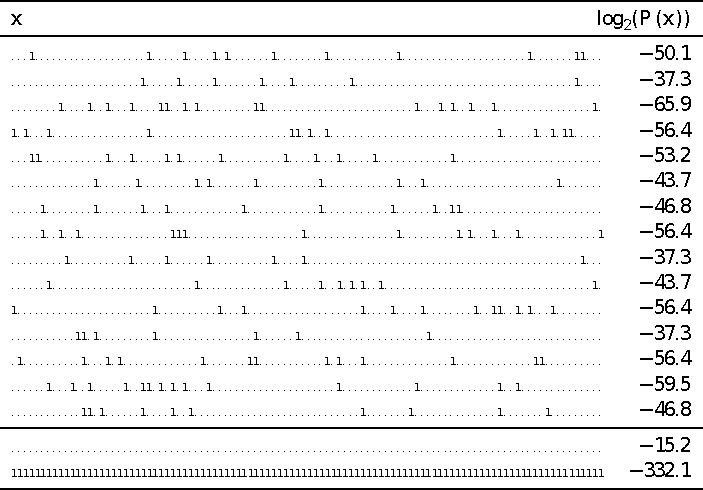
\includegraphics[width=\linewidth]{figures/seq100mackay.pdf}
  \caption{Sequências regadas por um ensaio de Bernoulli com $n=100$ e $P(X=1) = p = 0.1$.
        As 15 sequências superiores representam amostras típicas. As duas últimas sequências
        representam a sequência mais provável e a menos provável \parencite{mackay2003}.}
  \label{fig:seq100mackay}
\end{marginfigure}

Considere agora um ensaio de Bernoulli com $n = 100$ lançamentos, onde cada
lançamento $X_i$ é uma variável aleatória com $P(X_i = 1) = p = 0,1$ e
$P(X_i = 0) = 1-p = 0,9$. Nesse cenário, uma sequência 
$(x_1, x_2, \ldots, x_{100}) \in \{0,1\}^{100}$ tem probabilidade 
$P(x_1, \ldots, x_{100}) = p^k (1-p)^{n-k}$, onde $k = \sum_{i=1}^{100} x_i$ 
é o número de 1's na sequência. A \Cref{fig:seq100mackay} compara três tipos
de sequências: a mais provável, a menos provável e as sequências típicas.
A sequência mais provável é a sequência com 100 ocorrências de 0 (penúltima sequência
apresentada na \Cref{fig:seq100mackay}), já a sequência menos provável é aquela 
com 100 ocorrências de 1 (última sequência apresentada na \Cref{fig:seq100mackay}).
As sequências típicas são aquelas com probabilidade aproximadamente $2^{-nH(X)}$.
Para o exemplo em questão, temos $H = 0,4690$ e assim $\log (2^{-100 H(X)}) = -46.9$.
As 15 sequências apresentadas no parte superior da \Cref{fig:seq100mackay} representam
aquelas com $\log p(x_1,\ldots,x_n)$ próximo de $-46.9$, ou seja, sequências que
podemos considerar típicas (dado um determinado critério $\epsilon$).


\begin{figure}%
  \centering
  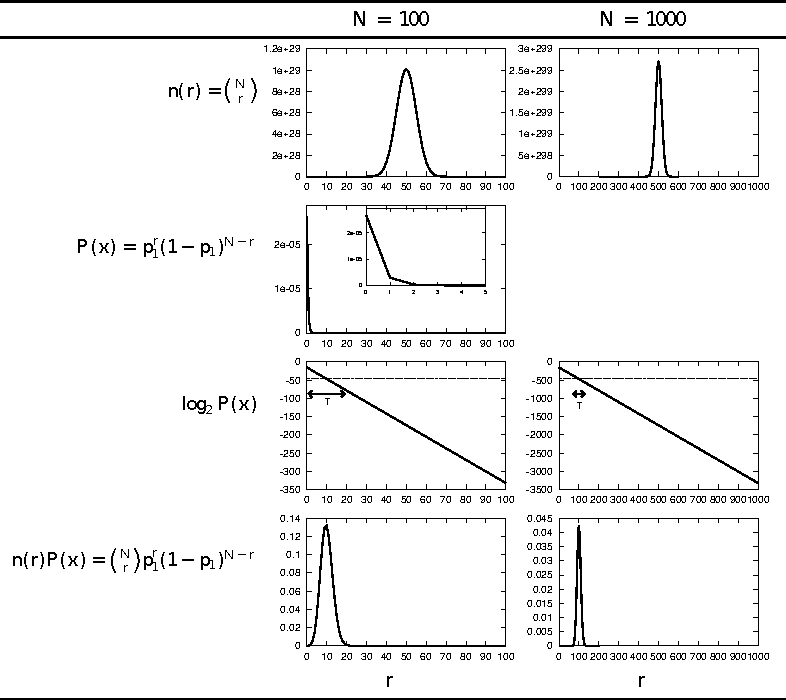
\includegraphics[width=\linewidth]{figures/seq100mackay2.pdf}
  \caption{Para $p=0.1$, $n=100$ e $n=1000$ os gráficos ilustram $n(r)$, o número de strings contendo 
    $r$ 1s; a probabilidade $P(x_{1:n})$ para uma string contendo $r$ 1s; a mesma probabilidade
    em escala logarítmica; e a probabilidade total $n(r) P(x_{1:n})$ de todas as strings contendo $r$ 1s \parencite{mackay2003}.
  }
  \label{fig:seq100mackay2}
\end{figure}

A \Cref{fig:seq100mackay2} ilustra o que ocorre quando $n$ cresce, fazendo assim
uma comparação para os casos $n=100$ e $n=1000$. Primeiramente, temos o número
de sequências de comprimento $n$ com $r$ ocorrências de 1's. Este número é dado
pelo coeficiente binomial. Nos extremos, existe apenas uma sequência com 100 zeros 
e uma sequência com 100 1's. No meio, teremos o pico, sequências com 50 ocorrências
de cada símbolo. Logo abaixo apresenta-se a probabilidade das sequências, que decai
rápidamente com o número de 1's presente na sequência. Por fim, temos o produto
dos dois gráficos anteriores, representando assim a probabilidade total das sequências
de um determinado tipo. Podemos observar, que o pico ocorre em sequências constituídas por
10\% de 1's. Verificamos ainda que este pico torna-se mais acentuado com o crescimento de $n$.
No limite, quando $n$ for muito grande, só ocorrerão sequências com 10\% de 1's.




\section{Codificação para o Conjunto Típico}

Após definirmos o que são sequências típicas e formalizarmos a propriedade da
equipartição assintótica, vamos agora abordar o problema de codificação
considerando a codificação de sequências típicas.  Como vimos que existe um
limite para o tamanho do conjunto típicos, iremos utilizar o número de bits
mínimo necessários para codificar as sequências quer pertençam a este conjunto.
As sequências remancessentes, contidas no conjunto não típico, podem ser
codificadas utilizando mais bits, sem que isto cause impacto significativo ao
código, uma vez que a probabilidade do conjunto típico é aproximadamente 1
(conforme \cref{prop2conjtip} do \Cref{thm:propconjtip}).

A ideia consiste em particionar o conjunto de sequencias em dois blocos:
conjunto típico $A_\epsilon^{(n)}$, e o seu complemento, o conjunto não típico 
$A_\epsilon^{(n)c} \triangleq \mathcal{X}^n \backslash A_\epsilon^{(n)}$.
Tais partições satisfazem $A_\epsilon^{(n)} \cap A_\epsilon^{(n)c} = \emptyset$, 
e $A_\epsilon^{(n)} \cup A_\epsilon^{(n)c} = \mathcal{X}^n$. A \Cref{fig:particao2}
ilustra o particionamento proposto.

\begin{marginfigure}%
  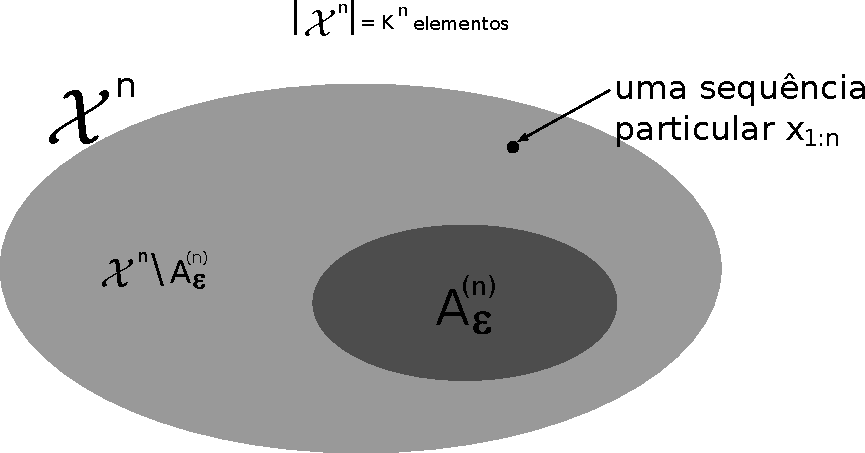
\includegraphics[width=\linewidth]{figures/particao2.pdf}
  \caption{Particionamento de $\mathcal{X}^n$ em dois conjuntos: $A_\epsilon^{(n)}$ e $A_\epsilon^{(n)c}$.}
  \label{fig:particao2}
\end{marginfigure}

Vamos então indexar os elementos de cada conjunto (conjunto típico e não-típico) separadamente.
O número de elementos do conjunto típico é $\vert A_\epsilon^{(n)} \vert \leq 2^{n(H+\epsilon)}$,
desta forma será necessário
\begin{equation}
  \lceil n(H+\epsilon) \rceil \leq n (H + \epsilon) + 1 \text{bits}
\end{equation}
para indexar os elementos deste conjunto.
Ainda, utilizaremos um bit extra para indicar se o elemento está no conjunto típico ou não, i.e.,
vamos utilizar uma sequência $(b_0,b_1,b_2,\ldots,b_{\lceil n(H+\epsilon) \rceil})$ onde
o primeiro bit indica se temos um elemento do conjunto típico ($b_0=0$) ou não
e os demais indexam o elemento do conjunto.
O número total de bits necessário para uma sequência típica será então $\leq n(H+\epsilon)+2$.

Para os elementos do conjunto não típico, vamos utilizar
\begin{equation}
  \lceil \log \vert \mathcal{X} \vert^n \rceil \leq n \log K + 1 \text{bits}.
\end{equation}
Então teremos um vetor binário da forma $(b_0,b_1,b_2,\ldots,b_{\lceil \log \vert \mathcal{X} \vert^n \rceil})$
onde $b_0=1$, indicando a atipicidade.
Assim, o número total de bits para indexar uma sequência atípica será $\leq n \log K + 2$.

Este código proposto é 1-pra-1, sendo fácil codificar e decodificar, dado o \textit{codebook}.
Para o conjunto não-típico $A_\epsilon^{(n)c}$ estamos utilizando mais bits do que o necessário,
já que $\vert A_\epsilon^{(n)c} \vert = \vert \mathcal{X}^n \vert - \vert A_\epsilon^{(n)} \vert = K^n - \vert A_\epsilon^{(n)} \vert \leq K^n$,
mas isto não importará, como veremos adiante.
O importante desta proposta de código é que as sequências típicas possuem um comprimento descritivo curto, aproximadamente $nH$.

\begin{definition}[Comprimento da palavra associada a uma sequência]
  O comprimento da palavra (\emph{codeword}) associada à sequência $x_{1:n}$ é denominado $l(x_{1:n})$.
\end{definition}
Assim, $l(X_{1:n})$ é uma variável aleatória, já que $X_{1:n}$ é uma variável aleatória.
Então $E l(X_{1:n}) = \sum_{x_{1:n}} p(x_{1:n}) l(x_{1:n})$ é o valor esperado do comprimento
do código. Queremos que ele seja o menor possível.

Suponha que $n$ seja grande suficiente de forma que $p(A_\epsilon^{(n)}) > 1 - \epsilon$, então
\begin{subequations}
  \begin{align}
    E l(X_{1:n}) &= \sum_{x_{1:n}} p(x_{1:n}) l(x_{1:n}) \\
                 &= \sum_{x_{1:n} \in A_\epsilon^{(n)}} p(x_{1:n}) l(x_{1:n}) + \sum_{x_{1:n} \in A_\epsilon^{(n)c}} p(x_{1:n}) l(x_{1:n}) \\
                 &\leq \sum_{x_{1:n} \in A_\epsilon^{(n)}} p(x_{1:n}) [n(H+\epsilon)+2] + \sum_{x_{1:n} \in A_\epsilon^{(n)c}} p(x_{1:n}) [n \log K + 2] \\
                 &= \underbrace{p(A_\epsilon^{(n)})}_{\leq 1} [n(H+\epsilon)+2] + \underbrace{p(A_\epsilon^{(n)c})}_{< \epsilon} [n \log K + 2] \\
                 &\leq n(H+\epsilon)+2 + \epsilon n \log K + \epsilon 2 \\
                 &= n [H + \underbrace{\epsilon + \epsilon \log K + \frac{2}{n} + \frac{2 \epsilon}{n}}_{\epsilon'} ] = n(H+\epsilon') ,
  \end{align}
\end{subequations}
onde definimos $\epsilon'$ como
\begin{equation}
  \epsilon' = \epsilon + \epsilon \log K + \frac{2}{n} + \frac{2 \epsilon}{n} .
\end{equation}
Podemos fazer $\epsilon'$ tão pequeno quanto queremos, fazendo $\epsilon$ pequeno e $n$ grande.
Desta forma, podemos fazer $n(H+\epsilon')$ tão próximo quanto quisermos de $nH$.

\begin{theorem}[Primeiro Teorema de Shannon]
Seja $X_{1:n}$ i.i.d. $\sim p(x)$, $\epsilon > 0$, então $\exists$ um código $f_n : \mathcal{X}^n \rightarrow \text{string binária}$
e um inteiro $n_{\epsilon}$, tal que o mapeamento seja um-pra-um (desta forma inversível sem erro), e
      \begin{equation}
      E[ \frac{1}{n} l(X_{1:n})] \leq H(X) + \epsilon
      \end{equation}
para todo $\epsilon > 0$ e todo $n \geq n_{\epsilon}$.
\end{theorem}

\begin{proof}
  A demonstração do Primeiro Teorema de Shannon usa a codificação de sequências típicas de maneira semelhante ao
  exemplo anterior.
\end{proof}


É interessante notar que a sequência mais provável não pertence ao conjunto
típico $A_\epsilon^{(n)}$. Isso ocorre porque o conjunto típico contém
sequências cujo histograma empírico é próximo da distribuição subjacente. A
tipicidade não está relacionada à probabilidade de uma única sequência ser a
maior. 

Dado que o conjunto típcio é tal que $P(A_\epsilon^{(n)}) \to 1$ à medida que
$n \to \infty$, ou seja, $A_\epsilon^{(n)}$ captura toda probabilidade, podemos
nos questionar se existe um conjunto ainda menor que também contenha
essencialmente `toda' a probabilidade.

\begin{definition}[Sequências asintoticamente iguais até a primeira ordem do expoente]\label{def:saiapoe}
A notação $a_n \circeq b_n$ indica que $a_n$ e $b_n$ são iguais até a primeira ordem do expoente,
ou seja, suas taxas de crescimento exponencial são as mesmas à medida que $n \to \infty$. 
Formalmente, isso significa que $\lim_{n \to \infty} \frac{1}{n} |\log a_n - \log b_n| = 0$, 
de modo que $\frac{1}{n} \log a_n \to \alpha$ e $\frac{1}{n} \log b_n \to \alpha$ 
para o mesmo $\alpha$. Para $n$ grande, $a_n$ e $b_n$ possuem aproximadamente o mesmo comportamento. 
\end{definition}

\begin{theorem}
Seja $X_{1:n}$ uma sequência i.i.d. $\sim p(x)$. Para $\delta < \sfrac{1}{2}$ e qualquer $\delta' > 0$,
se $P(B_{\delta}^{(n)}) > 1 - \delta$, então
\begin{equation}
\frac{1}{n} \log \vert B_{\delta}^{(n)} \vert >  H - \delta',
\end{equation}
se $n$ é grande suficiente. Teremos assim
\begin{equation}
\vert B_{\delta}^{(n)} \vert > 2^{n(H-\delta')} \approx 2^{nH}
\end{equation}

Usando a \Cref{def:saiapoe}, podemos então reescrever o teorema anterior da seguinte forma:

Se $\delta_n \rightarrow 0$ e $\epsilon_n \rightarrow 0$, então teremos
\begin{equation}
\vert B_{\delta_n}^{(n)} \vert \circeq \vert A_{\epsilon_n}^{(n)} \vert \circeq 2^{nH}.
\end{equation}
\end{theorem}
\begin{proof}
Seja $X_1, X_2, \ldots, X_n$ i.i.d. $\sim p(x)$. Seja $B_{\delta}^{(n)} \subset \mathcal{X}^n$ tal que
$\Pr(B_{\delta}^{(n)}) > 1 - \delta$. Fixe $\epsilon < \sfrac{1}{2}$.
Dados dois subconjuntos quaisquer $A$ e $B$ tais que $\Pr(A) > 1 - \epsilon_1$ e $\Pr(B) > 1 - \epsilon_2$.
Seja $A^c$ o complemento de $A$ e $B^c$ o complemento de $B$, então
\begin{equation}
P(A^c \cup B^c) \leq P(A^c) + P(B^c) .
\end{equation}

Como $P(A) > 1 - \epsilon_1$, teremos $P(A^c) \leq \epsilon_1$. De forma similar, $P(B^c) \leq \epsilon_2$.
Poderemos assim escrever
\begin{subequations}
\begin{align}
P(A \cap B) &= 1 - P(A^c \cup B^c) \\
        &\geq 1 - P(A^c) - P(B^c) \\
        &\geq 1 - \epsilon_1 - \epsilon_2.
\end{align}
\end{subequations}

Podemos reescrever a desigualdade anterior como
\begin{equation}
\Pr(A_{\epsilon}^{(n)} \cap B_{\delta}^{(n)}) \geq 1 - \epsilon - \delta .
\end{equation}

A probabilidade de um conjunto é dada pela soma das probabilidades de todos os elementos (sequências) neste conjunto, logo teremos
\begin{equation}
\Pr(A_{\epsilon}^{(n)} \cap B_{\delta}^{(n)}) = \sum_{x^n \in A_{\epsilon}^{(n)} \cap B_{\delta}^{(n)}} p(x^n)
\end{equation}
A probabilidade dos elementos no conjunto típico é limitada por $2^{-n(H-\epsilon)}$.

Desta forma teremos
\begin{subequations}
\begin{align}
 1 - \epsilon - \delta &\leq \Pr(A_{\epsilon}^{(n)} \cap B_{\delta}^{(n)}) \\
                &= \sum_{x^n \in A_{\epsilon}^{(n)} \cap B_{\delta}^{(n)}} p(x^n) \\
                &\leq \sum_{x^n \in A_{\epsilon}^{(n)} \cap B_{\delta}^{(n)}} 2^{-n(H-\epsilon)} \\
                &= \vert A_{\epsilon}^{(n)} \cap B_{\delta}^{(n)} \vert 2^{-n(H-\epsilon)} \\
                &\leq \vert B_{\delta}^{(n)} \vert 2^{-n(H-\epsilon)},
\end{align}
\end{subequations}
onde utilizamos $A_{\epsilon}^{(n)} \cap B_{\delta}^{(n)} \subseteq B_{\delta}^{(n)}$.

Poderemos reescrever então da seguinte forma,
\begin{equation}
\vert B_{\delta}^{(n)} \vert  >  2^{n(H-\epsilon)} ,
\end{equation}
onde $\epsilon > 0$.
\end{proof}











\section{Método de Típos}

O método de tipos refina a abordagem das sequências típicas, oferecendo uma
análise mais estruturada das propriedades assintóticas. O método de tipos
considera todas as possíveis distribuições empíricas (ou `tipos') que
sequências $x_{1:n}$ podem ter, agrupando-as em conjuntos de sequências que
compartilham um mesmo histograma empírico $\hat{p}_n(x_{1:n})$, ou
$P_{x_{1:n}}$. O conjunto de sequências de comprimento $n$ pode ser
particionado em subconjuntos de sequências de tipos distintos. Na AEP, o método
de tipos confirma que o número de sequências típicas é $\circeq 2^{nH(X)}$.
Vamos então estabelecer algumas definições.

\begin{definition}[Tipo]
  Seja $X_1, X_2, \ldots, X_n \equiv X_{1:n}$ uma amostra de comprimento $n$ de uma variável aleatória discreta $D$-ária.
  Então $x_i \in \mathcal{X}$ e o tamanho do alfabeto é $D=\vert \mathcal{X} \vert$, e $\mathcal{X}=\{a_1, a_2, \ldots, a_D\}$.
  Definimos a seguinte estatística, o histograma empírico da amostras, também chamado tipo da amostra:
  \begin{equation}
  P_{x_{1:n}} \triangleq \left( \frac{n(a_1|x_{1:n})}{n}, \frac{n(a_2|x_{1:n})}{n}, \ldots, \frac{n(a_D|x_{1:n})}{n} \right)
  \end{equation}
  onde $n(a_i|x_{1:n})$ representa o número de ocorrências do símbolo $a_i$ na amostra $x_{1:n}$.
\end{definition}
Note que $P_{x_{1:n}}$ pode ser considerado como uma função massa probabilidade.
Um tipo $\hat{p}$ é uma função de massa de probabilidade sobre $S_X$, 
definido como o histograma empírico $\hat{p}(a) = \frac{k_a}{n}$, 
onde $k_a = \sum_{i=1}^n \mathbb{I}\{x_i = a\}$ é o número de ocorrências do símbolo $a \in S_X$ na sequência, 
e $\sum_{a \in S_X} k_a = n$.

\begin{definition}[Conjunto de Tipos]
    O Conjunto de Tipos $\mathcal{P}_n$, ou $\mathcal{P}_n (\mathcal{X})$, para sequências de comprimento $n$ sobre um alfabeto finito $\mathcal{X}$ 
    é o conjunto de todas as possíveis distribuições empíricas (ou tipos) que podem ser formadas 
    por sequências $(x_1, x_2, \ldots, x_n) \in \mathcal{X}^n$.
\end{definition}
\begin{example}[Ensaio de Bernoulli]
Para sequências de comprimento $n$ geradas a partir de um ensaio de Bernoulli com alfabeto $\mathcal{X} = \{0,1\}$,
teremos o seguinte conjunto de tipos:
\begin{equation}\label{eq:exconjtiposbernoulli}
\mathcal{P}_n (\mathcal{X}) = \left\{ \left( \frac{0}{n}, \frac{n}{n} \right), \left( \frac{1}{n} , \frac{n-1}{n} \right), \ldots, \left( \frac{n}{n}, \frac{0}{n} \right)\right\}
\end{equation}
onde existem $n+1$ tipos (histogramas empíricos). O primeiro tipo em \ref{eq:exconjtiposbernoulli} representa
a sequência sem nenhuma ocorrência de zeros e $n$ ocorrências de uns; o segundo tipo representa 
as sequências com apenas uma ocorrência de zero e $n-1$ ocorrência de uns; e o último tipo
representa a sequência com $n$ ocorrência de zeros e nenhuma ocorrência de uns.
\end{example}


\begin{definition}[Classe de Tipo]
    A Classe de Tipo $T(P)$, ou $T(\hat{p})$, associada a um tipo $\hat{p} \in \mathcal{P}_n(\mathcal{X})$, 
    para sequências de comprimento $n$ sobre um alfabeto finito $\mathcal{X}$, 
    é o conjunto de todas as sequências $(x_1, x_2, \ldots, x_n) \in \mathcal{X}^n$ 
    que compartilham um mesmo histograma empírico $\hat{p}$, ou $P$.
    \begin{equation}
      T(P) \triangleq \{ x_{1:n} \in \mathcal{X}^n : P_{x_{1:n}} = P \} .
    \end{equation}
\end{definition}
\begin{example}[Ensaio de Bernoulli]
Para o caso do ensaio de Bernoulli, vejamos alguns exemplos de classe de tipo.

Para o tipo $P = \left( \frac{0}{n}, \frac{n}{n} \right)$, a classe de tipo $T(P)$ 
possui apenas uma sequência:
\begin{equation}
    T(P) = \{ 111\cdots{}11 \} .
\end{equation}

Para o tipo $P = \left( \frac{1}{n} , \frac{n-1}{n} \right)$, a classe de tipo $T(P)$
possui $n$ sequências:
\begin{equation}
    T(P) = \{ 011\cdots{}11, 101\cdots{}11, \ldots, 111\cdots{}01, 111\cdots{}10 \} .
\end{equation}

Para o tipo $P = \left( \frac{n}{n}, \frac{0}{n} \right)$, a classe de tipo $T(P)$
possui apenas uma sequência:
\begin{equation}
    T(P) = \{ 000\cdots{}00 \} .
\end{equation}
\end{example}


Como mencionado anteriormente, o conjunto de todas sequências $\mathcal{X}^n$
pode ser particionado em diferentes conjuntos $T(P_i)$, com $P_i \in \mathcal{P}_n$,
o conjunto de todos os tipos, ou seja, $\mathcal{P}_n = \{ P_1, P_2, \ldots, P_{\vert \mathcal{P}_n \vert} \}$.
As partições são disjuntas
\begin{equation}
    T(P_i) \cap T(P_j) = \emptyset, \forall i,j \in \{1, \ldots, \vert \mathcal{P}_n \vert\} \text{ e } i \neq j,
\end{equation}
e o particionamento é exaustivo
\begin{equation}
  \bigcup_{P \in \mathcal{P}_n} T(P) = \mathcal{X}^n.
\end{equation}
Este particionamento é ilustrado na \Cref{fig:particao-Xn2}.

\begin{marginfigure}%
  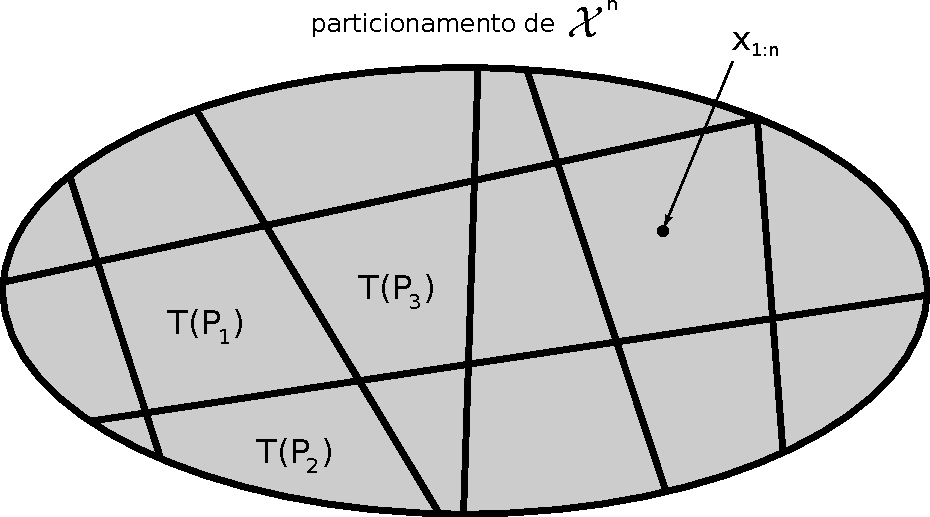
\includegraphics[width=\linewidth]{figures/particao-Xn2.pdf}
  \caption{Particionamento do espaço de sequências de comprimento $n$.}
  \label{fig:particao-Xn2}
\end{marginfigure}


No exemplo do ensaio de Bernoulli é fácil constatar quantos tipos distintos existem.
O \Cref{thm:numtiposn} a seguir usa o método estrela traço da análise combinatória para determinar
o número de tipos existentes. Vejamos então primeiramente o teorema da análise combinatória.

\begin{theorem}[Método Estrela Traço]
    Suponha que $n$ estrelas que devem ser organizadas em $k$ recipientes, podendo inclusive
    ter recipiente vazio.
    Neste caso, o número de maneiras de fazer tal organização é dado por
    \begin{equation}
	\binom{n+k-1}{k-1}
    \end{equation}
\end{theorem}
\begin{proof}
Este problema é o mesmo que incluir $k-1$ traços para separar uma sequência de $n$ estrelas.
Os traços podem ser inseridos em qualquer posição, inclusive sem existir estrelas entre eles,
como por exemplo, com $n=7$ e $k=4$:
$$\star \star \star \star \quad | \quad | \quad \star \quad | \quad \star \star$$
Note que, neste problema temos $n+k-1$ símbolos (estrelas e traços) para serem incluídos, dos
quais $k-1$ são escolhidos para serem traços. Desta forma existem $\tbinom{n+k-1}{k-1}$
formas de dispor estes símbolos.
\end{proof}

\begin{theorem}[Número de tipos existentes]\label{thm:numtiposn}
 Para sequências de comprimento $n$, em um alfabeto $\mathcal{X}$, o número de tipos é dado por
 \begin{equation}\label{eq:number-of-types}
 \vert \mathcal{P}_n \vert = {n + \vert \mathcal{X} \vert - 1 \choose \vert \mathcal{X} \vert - 1}
 \end{equation}
\end{theorem}
\begin{proof}
Um histograma empírico pode ser visto como uma variação do problema estrela-traço.
Se temos um alfabeto com $\vert\mathcal{X}\vert = D$ símbolos,
o Conjunto de Tipos $\mathcal{P}_n$ contém todas as possíveis distribuições empíricas $\hat{p}$
para sequências de comprimento $n$ sobre o alfabeto $\mathcal{X}$.
Um tipo $\hat{p}$ é uma função de massa de probabilidade tal que $\hat{p}(a) = \sfrac{k_a}{n}$,
onde $k_a$ é o número de ocorrências do símbolo $a \in \mathcal{X}$, e
$\sum_{a \in \mathcal{X}} k_a = n$. Assim, $k_a \in \{0,1, \ldots, n\}$, e a restrição
é que a soma de todos $k_a$'s deve ser igual a $n$, o comprimento da sequência.
Cada tipo $\hat{p}$ é definido pela ênupla $(k_{a_1}, k_{a_2}, \ldots, k_{a_D})$, e cada
uma delas corresponde a uma forma de organização no problema de estrelas e traços.
\end{proof}


Embora tenhamos uma fórmula fechada para o número de tipos, \Cref{eq:number-of-types},
iremos encontrar um limite superior para $\vert \mathcal{P}_n \vert$,
que, embora seja um limite relativamente largo, é mais fácil de manipular e suficiente 
para muitas demonstrações teóricas. 

\begin{theorem}[Limite no número de tipos]
 O número de tipos para sequências de comprimento $n$ em um alfabeto $\mathcal{X}$ é limitado por
 \begin{equation}\label{eq:number-of-types-bound}
 \vert \mathcal{P}_n \vert \leq (n+1)^{\vert \mathcal{X} \vert} .
 \end{equation}
\end{theorem}

\begin{proof}
 O numerador de cada entrada em um tipo pode assumir $(n+1)$ valores distintos (de $0$ a $n$).
 Existem $\vert \mathcal{X} \vert$ entradas em um tipo, e portanto a mesma quantidade de numeradores.
 Os valores dos numeradores interagem entre si (a soma de todos deve ser igual a $n$), mas podemos
 achar um limite superior desconsiderando esta interação.
 \begin{equation}
 \vert \mathcal{P}_n \vert \leq \underbrace{(n+1)\times(n+1)\times\ldots\times(n+1)}_{\vert \mathcal{X} \vert \text{ vezes}} = (n+1)^{\vert \mathcal{X} \vert} .
 \end{equation}
\end{proof}

É importante notar na \Cref{eq:number-of-types-bound} que existe no máximo um número polinomial em
$n$ de tipos de sequencias de comprimento $n$. Entretanto, sabemos que o número de sequências cresce com $n$,
$\vert \mathcal{X} \vert^n$. Com $n$ grande suficiente, eventualmente, teremos que apenas um único tipo
(o tipo das sequências típicas) conterá todas as sequências, como será demonstrado no \Cref{thm:teocodshannontipos}.


Para sequências geradas por uma fonte i.i.d., a probabilidade de uma sequência
$(x_1, x_2, \ldots, x_n)$ depende apenas do seu tipo e não da sequência específica.
Isso significa que todas as sequências em uma mesma classe de tipo, ou seja,
sequências que compartilham um mesmo histograma empírico, têm a mesma probabilidade.

\begin{theorem}[Probabilidade Depende do Tipo]
Seja $X_1, X_2, \ldots, X_n$ i.i.d. $\sim Q(x)$, com $Q$ arbitrário, e extensão
$Q^n(x_{1:n}) = \prod_i Q(x_i)$, a probabilidade da sequencia depende apenas do tipo, ou seja,
a probabilidade é `independente' da sequencia, dado o tipo e $Q$, isto é,
\begin{equation}
Q^n(x_{1:n}) = 2^{-n[ H(P_{x_{1:n}}) + D(P_{x_{1:n}}||Q) ]} .
\end{equation}
\end{theorem}

\begin{proof}
\begin{subequations}
\begin{align}
  Q^n(x_{1:n}) &= \prod_{i=1}^{n} Q(x_i) = \prod_{a \in \mathcal{X}} Q(a)^{n(a \mid x_{1:n})} \\
        &= \prod_{a \in \mathcal{X}} Q(a)^{n P_{x_{1:n}}(a) } = \prod_{a \in \mathcal{X}} 2^{ \left\{ n P_{x_{1:n}}(a) \log Q(a) \right\} } \\
        &= \prod_{a \in \mathcal{X}} 2^{ n \left\{  P_{x_{1:n}}(a) \log Q(a) \KeepStyleUnderBrace{ -P_{x_{1:n}}(a) \log P_{x_{1:n}}(a) + P_{x_{1:n}}(a) \log P_{x_{1:n}}(a) }_{=0} \right\} } \\
        &= 2^{n \sum_{a \in \mathcal{X}}  \left( -P_{x_{1:n}}(a) \log \frac{P_{x_{1:n}}(a)}{Q(a)} + P_{x_{1:n}}(a) \log P_{x_{1:n}}(a) \right)  } \\
        &= 2^{-n \left( D(P_{x_{1:n}} \mid \mid Q) + H( P_{x_{1:n}} ) \right) } .
\end{align}
\end{subequations}
\end{proof}

Se $Q$ é uma distribuição racional (i.e., um tipo possível) e se $x_{1:n} \in T(Q)$, então
\begin{equation}
Q^n(x_{1:n}) = 2^{-n H(Q)} .
\end{equation}
Se $Q$ for irracional, podemos fazer $D(P_{x_{1:n}} \mid \mid Q)$  tão pequeno quando desejável,
fazendo $n$ grande suficiente.

No método de tipos, uma questão natural é identificar qual classe de tipo
tem a maior probabilidade total quando as sequências são geradas por uma 
determinada distribuição. Intuitivamente, esperamos que a classe de tipo
mais provável seja aquela cujo histograma empírico esteja mais próximo 
da distribuição geradora.

\begin{lemma}[Classe de Tipo com maior probabilidade]
Dada a distribuição geradora $Q = P \in \mathcal{P}_n$, teremos que $T(P)$ possui a maior probabilidade. Isto é
\begin{equation}
  P^n(T(P)) \geq P^n(T(\hat{P})) , \ \forall \hat{P} \in \mathcal{P}_n .
\end{equation}
\end{lemma}
\begin{proof}
  \begin{subequations}
  \begin{align}
  \frac{P^n(T(P))}{P^n(T(\hat{P}))} &= \frac{\vert T(P) \vert \prod_{a \in \mathcal{X}} P(a)^{nP(a)} }{ \vert T(\hat{P}) \vert \prod_{a \in \mathcal{X}} P(a)^{n\hat{P}(a)}  } \\
        &= \frac{ { n \choose nP(a_1) \ nP(a_2) \ \ldots \ nP(a_D) } \prod_{a \in \mathcal{X}} P(a)^{nP(a)} }{ { n \choose n\hat{P}(a_1) \ n\hat{P}(a_2) \ \ldots \ n\hat{P}(a_D) } \prod_{a \in \mathcal{X}} P(a)^{n\hat{P}(a)}  } \\
        &= \prod_{a \in \mathcal{X}} \frac{ [n\hat{P}(a)]! }{[nP(a)]!} P(a)^{n(P(a)-\hat{P}(a))} \\
	&\geq \prod_{a \in \mathcal{X}} (nP(a))^{n(\hat{P}(a)-P(a))} P(a)^{n(P(a)-\hat{P}(a))} \label{eq:demctmp}\\
        &= \prod_{a \in \mathcal{X}} n^{n(\hat{P}(a)-P(a))} \\
	&\geq \prod_{a \in \mathcal{X}} n^{n(\hat{P}(a)-P(a))} \\
        &= n^{n\left[ \sum_{a \in \mathcal{X}} \hat{P}(a) - \sum_{a \in \mathcal{X}} P(a) \right]} \\
        &= n^{n(1-1)} = 1 ,
  \end{align}
  \end{subequations}
  onde em \ref{eq:demctmp} utilizamos que $\frac{m!}{n!} \geq n^{m-n}$, para $m$ e $n$ inteiros não negativos\footnote{
    Sejam $m$ e $n$ inteiros não negativos, então $\frac{m!}{n!} \geq n^{m-n}$.
    Se $m>n$, então $\frac{m!}{n!} = m(m-1) \ldots (n+1) \geq n^{m-n}$.
    Se $m<n$, então $\frac{m!}{n!} = \frac{1}{n(n-1)\ldots(m+1)} \geq \frac{1}{n^{n-m}}$.
    Se $m=n$, $\frac{m!}{n!} = 1 = n^0$.
  }.
  Por fim, temos que $P^n(T(P)) \geq P^n(T(\hat{P}))$.
\end{proof}


O tamanho de uma classe de tipo $T(P)$ pode ser determinado pelos coeficientes multinomiais.
Cada sequência $x_{1:n} \in T(P)$ possui exatamente $nP(a)$ ocorrências de cada símbolo $a \in \mathcal{X}$.
O número de sequências corresponde ao número de maneiras de permutar os símbolos de acordo com o número de ocorrência de cada símbolo.

\begin{lemma}[Tamanho da Classe de Tipo]
    Seja $P \in \mathcal{P}_n$, um tipo para sequências de comprimento $n$ sobre um alfabeto finito $\mathcal{X}$,
    de tamanho $D = \vert\mathcal{X}\vert$, 
    e seja $T(P)$ a classe de tipo associada, ou seja, o conjunto de todas as sequências $x_{1:n} \in \mathcal{X}^n$
    com histograma empírico $P$. Então o tamanho de $T(P)$ é dado por
    \begin{equation}\label{eq:tamclasstipo}
	\vert T(P) \vert = { n \choose nP(a_1) \ nP(a_2) \ \ldots \ nP(a_D) } = \frac{n!}{\prod_{a \in \mathcal{X}} (nP(a))!} .
    \end{equation}
\end{lemma}
\begin{proof}
    Cada sequência em $T(P)$ tem exatamente $nP(a)$ ocorrências de cada símbolo $a \in \mathcal{X}$,
    com $\sum_{a \in \mathcal{X}} (nP(a)) = n$.
    O número de sequências distintas é o número de maneiras de permutar os $n$ símbolos,
    considerando que as permutações dentro de cada símbolo não geram sequências distintas. 
    Assim, o número de permutações distintas é o coeficiente multinomial, como dado na \Cref{eq:tamclasstipo}.
\end{proof}

Novamente, apesar de termos o resultado exato, dado pela \Cref{eq:tamclasstipo}, em muitas situação
é mais prático utilizarmos limites que nos forneçam uma notação mais intuitiva e prática
para utilização em outras demonstrações. Veremos então a seguir os limites superior e inferior
para o tamanho da classe de tipo.


\begin{theorem}[Limites no tamanho da Classe de Tipo]\label{thm:limtamclasstip}
Dado um tipo $P \in \mathcal{P}_n$, temos
\begin{equation}\label{eq:limtamclasstip}
\frac{1}{(n+1)^{\vert \mathcal{X} \vert}} 2^{nH(P)} \leq \vert T(P) \vert \leq 2^{nH(P)} .
\end{equation}
\end{theorem}
\begin{proof}[Demonstração (limite superior)]
\begin{subequations}
\begin{align}
  1 &\geq P^{n} (T(P)) = \sum_{x_{1:n} \in T(P)} P^{n} (x_{1:n}) = \sum_{x_{1:n} \in T(P)} 2^{-nH(P)} \\
    &= \vert T(P) \vert 2^{-nH(P)}
\end{align}
\end{subequations}
\end{proof}
\begin{proof}[Demonstração (limite inferior)]
\begin{subequations}
\begin{align}
  1 &= \sum_{Q \in \mathcal{P}_n} P^n (T(Q)) \leq \sum_{Q \in \mathcal{P}_n} \max_{R \in \mathcal{P}_n} P^n (T(R)) \\
       &= \sum_{Q \in \mathcal{P}_n} P^n (T(P)) \leq (n+1)^{\vert \mathcal{X} \vert} P^n (T(P)) \label{eq:demliminftamclasstip}\\
      &= (n+1)^{\vert \mathcal{X} \vert} \sum_{x_{1:n} \in T(P)} P^n (x_{1:n}) \\
      &= (n+1)^{\vert \mathcal{X} \vert} \sum_{x_{1:n} \in T(P)} 2^{-nH(P)} \\
      &\leq (n+1)^{\vert \mathcal{X} \vert} \sum_{x_{1:n} \in T(P)} 2^{-nH(P)} \\
      &= (n+1)^{\vert \mathcal{X} \vert} \vert T(P) \vert 2^{-nH(P)} ,
\end{align}
\end{subequations}
onde em \ref{eq:demliminftamclasstip} utilizamos
\begin{equation}
  P = \argmax_{R \in \mathcal{P}_n} P^n (T(R)) .
\end{equation}
Ao final, obtemos
\begin{equation}
\vert T(P) \vert \geq \frac{1}{(n+1)^{\vert \mathcal{X} \vert}} 2^{nH(P)} .
\end{equation}
\end{proof}

Para o caso binário, $\mathcal{X} = \{0,1\}$, o \Cref{thm:limtamclasstip}
nos fornece os seguintes seguintes limites para o tamanho da classe de tipo:
\begin{equation}
  \frac{1}{(n+1)^2} 2^{nH(\frac{k}{n})} \leq {n \choose k} \leq 2^{nH(\frac{k}{n})} ,
\end{equation}
entretanto, o limite inferior pode ser ainda mais restrito, fornecendo assim
\begin{equation}
  \frac{1}{(n+1)} 2^{nH(\frac{k}{n})} \leq {n \choose k} \leq 2^{nH(\frac{k}{n})} .
\end{equation}

Os limites superior e inferior para o tamanho de uma classe de tipo $T(P)$, dados no
\Cref{thm:limtamclasstip}, podem ser utilizados para derivar limites correspondentes na probabilidade total
da classe de tipo $Q^n(T(P))$, onde $Q$ é a distribuição subjacente da fonte i.i.d. que gera as sequências.
Um resultado importante é que qualquer outro tipo que seja menos próximo de $Q$ (em termos de divergência de Kullback-Leibler)
terá sua probabilidade decrescendo exponencialmente com $n$, decrescendo assim mais rapidamente que o tipo mais provável.

\begin{theorem}[Limites da probabilidade da classe de tipo]
 Para qualquer $P \in \mathcal{P}_n$ e seja $Q$ a distribuição subjacente da fonte i.i.d., a probabilidade da classe de tipo
$T(P)$ sob $Q^n$ é tal que $Q^n(T(P)) \circeq 2^{-n D(P \mid \mid Q)}$. Especificamente, temos os limites
\begin{equation}
 \frac{1}{(n+1)^{\vert \mathcal{X} \vert}} 2^{-n D(P \mid \mid Q)} \leq Q^n(T(P)) \leq 2^{-nD(P \mid \mid Q)} .
\end{equation}
\end{theorem}
\begin{proof}
  \begin{subequations}
   \begin{align}
   Q^n(T(P)) &= \sum_{x_{1:n} \in T(P)} Q^n(x_{1:n}) = \sum_{x_{1:n} \in T(P)} 2^{-n (D(P \mid \mid Q) + H(P))} \\
             &= \vert T(P) \vert 2^{-n (D(P \mid \mid Q) + H(P))}
   \end{align}
  \end{subequations}
  para completar a demonstração, os limites do tamanho da classe de tipo dados pela \Cref{eq:limtamclasstip}.
\end{proof}


Iremos agora rever a definição de conjunto típico, utilizando a formalização do métodos de tipos.
\begin{definition}[Conjunto Típico]
  Seja $X_1, X_2, \ldots, X_n$ i.i.d. $\forall i$, $X_i \sim Q(x)$. Então o conjunto típico é definido como
  \begin{equation}
    T^{\epsilon}_{Q} = \{ x_{1:n} : D(P_{x_{1:n}} \mid \mid Q) \leq \epsilon \} .
  \end{equation}
\end{definition}

Podemos agora analizar a probabilidade do conjunto típico.
\begin{theorem}[Probabilidade do Conjunto Típico]
  Sejam $X_1, X_2, \ldots, X_n$ i.i.d. $\forall i$, $X_i \sim Q(x)$. A probabilidade do complemento
  do conjunto típico $\overline{T}^{\epsilon}_Q$ é dada por
  \begin{equation}
    Q(\overline{T}^{\epsilon}_Q) = Q( \{ x_{1:n} : D(P_{x_{1:n}} \mid\mid Q) > \epsilon  \} ) \leq 2^{-n (\epsilon - \vert \mathcal{X} \vert \frac{\log (n+1)}{n})} .
  \end{equation}
  Dessa forma,
  \begin{equation}
    D(P_{x_{1:n}} \mid\mid Q) \xrightarrow{p} 0 \text{, quando } n \rightarrow \infty ,
  \end{equation}
  ou seja, a divergência entre $P_{x_{1:n}}$ e $Q$ converge em probabilidade para zero quando $n$ é grande suficiente.
  \end{theorem}
  \begin{proof}
  \begin{subequations}
  \begin{align}
  Q(\overline{T}^{\epsilon}_Q) &= \sum_{P \in \mathcal{P}_n : D(P \mid\mid Q) > \epsilon} Q^n (T(P)) \\
        &\leq \sum_{P \in \mathcal{P}_n : D(P \mid\mid Q) > \epsilon} 2^{-n D(P\mid\mid Q)} \\
        &\leq \sum_{P \in \mathcal{P}_n : D(P \mid\mid Q) > \epsilon} 2^{-n \epsilon} \\
        &\leq (n+1)^{\vert \mathcal{X}  \vert} 2^{-n \epsilon} = 2^{-n \left( \epsilon - \vert \mathcal{X} \vert \frac{\log (n+1)}{n}  \right)}
  \end{align}
  \end{subequations}
  então a probabilidade vai para zero quando $n \rightarrow \infty$, e desta forma a probabilidade do conjunto típico vai para $1$ quando $n \rightarrow \infty$.
  \end{proof}
Os tipos que divergem (KL) mais do que $\epsilon$ da distribuição subjacente $Q$ terão probabilidade decrescente.
Para $n$ grande, o conjunto típico acaba sendo a única coisa que ocorre com uma probabilidade não evanescente.









Dizemos que uma codificação de fonte é universal quando ela não depende da distribuição fonte.
Seria possível criar um código universal que atinja o limite da entropia, ou seja, uma taxa $R>H(Q)$
(em bits por símbolo), onde $H(Q)$ é a entropia da distribuição subjacente $Q$?
O método de tipos oferece uma abordagem para formalizar o teorema de Shannon, 
permitindo uma análise mais refinada das sequências com base em seus histogramas empíricos.
Existem no máximo $2^{nH(P)}$ sequências do tipo $P$. Podermos utilizar $nH(P)$ bits para
representar tais sequencias. Se $R > H(P)$, podemos utilizar $nR$ bits para representar estas sequências.
Quando $n$ cresce, apenas os tipos $P$ `próximos' de $Q$ irão ocorrer.

A \Cref{fig:Mncodes2} ilustra um codificador de blocos que associa cada uma das $M$ sequências de $n$ de símbolos
da fonte a uma sequência binária de comprimento $m$.
Neste codificadador de blocos, cada sequências de $n$ símbolos é codificada conjuntamente
associando a ela uma palavra a cada. O codificador faz o mapeamento de sequências de tamanho $n$ produzidas pela fonte em
sequências de $m$ bits.
$M$ é o número de possíveis mensagens e também o número de palavras do \emph{codebook} do codificador.
\begin{marginfigure}%
  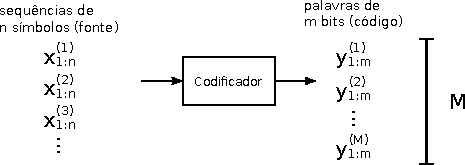
\includegraphics[width=\linewidth]{figures/Mncodes2.pdf}
  \caption{Codificador $(M,n)$, onde $M$ representa o número de mensagens e $n$ o comprimento das sequências.}
  \label{fig:Mncodes2}
\end{marginfigure}

\begin{definition}[Código de Bloco com Taxa Fixa $R$]
Seja $X_1, X_2, \ldots, X_n \sim Q$, i.i.d. mas $Q$ desconhecido. A função do codificador
e decodificador são definidas a seguir:
  \begin{equation}
  \text{codificador: } f_n : \mathcal{X}^n \rightarrow \{1,2,\ldots,2^{nR}\}
  \end{equation}
  \begin{equation}
  \text{decodificador: } \phi_n : \{1,2,\ldots,2^{nR}\} \rightarrow \mathcal{X}^n
  \end{equation}
e a probabilidade de erro
  \begin{equation}
  P_e^{(n)} = Q^n (\{ x_{1:n} : \phi (f_n (x_{1:n})) \neq x_{1:n} \}) .
  \end{equation}
\end{definition}

\begin{definition}[Código de Bloco Universal de Taxa $R$]
  Um código de bloco de taxa $R$ para um fonte é dito universal se a função $f_n$ e $\phi_n$
  não depender da distribuição $Q$ e se
  \begin{equation}
    P_e^{(n)} \rightarrow 0 \text{ quando } n \rightarrow \infty \text{ sempre que } H(Q) < R .
  \end{equation}
\end{definition}

Veremos que, se $R > H(Q)$, então existe uma sequência (em $n$) de códigos com erro evanescente.
Por outro lado, se $R < H(Q)$ a probabilidade de erro vai pra $1$.

Na demonstração do \Cref{thm:teocodshannontipos} utilizaremos ainda a definição de simplex probabilístico.
\begin{definition}[Simplex Probabilístico]
  O Simplex Probabilístico em $\RealNumber^m$ é o conjunto de pontos
  $x_{1:m} = (x_1, x_2, \ldots, x_m) \in \RealNumber^m$ tal que $x_i \geq 0$, $\sum_{i=1}^{m} x_i = 1$.
\end{definition}

\begin{example}[Simplex Probabilístico com $m=2$]
  O Simplex probabilístico será o conjunto de pontos
  \begin{equation}
  \{ (x_1, x_2)  :  x_1 \geq 0 , x_2 \geq 0 , x_1 + x_2 = 1 \} ,
  \end{equation}
  representado na \Cref{fig:prob-simplex-2}.
    \begin{marginfigure}
    \centering
    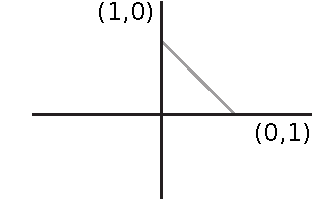
\includegraphics[width=\textwidth]{figures/prob-simplex-2.pdf}
    \caption{Simplex probabilístico para $m=2$.}
    \label{fig:prob-simplex-2}
    \end{marginfigure}
\end{example}

 \begin{example}[Simplex Probabilístico com $m=3$]
  O Simplex probabilístico será o conjunto de pontos
  \begin{equation}
  \{ (x_1, x_2, x_3)  :  x_1 \geq 0 , x_2 \geq 0 , x_3 \geq 0 , x_1 + x_2 + x_3 = 1 \}
  \end{equation}
  representado na \Cref{fig:prob-simplex-3} e com alguns pontos em destaque na \Cref{fig:prob-simplex-3t}.
    \begin{marginfigure}
    \centering
    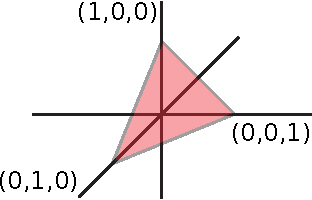
\includegraphics[width=\textwidth]{figures/prob-simplex-3.pdf}
    \caption{Simplex probabilístico para $m=3$.}
    \label{fig:prob-simplex-3}
    \end{marginfigure}

    \begin{marginfigure}
    \centering
    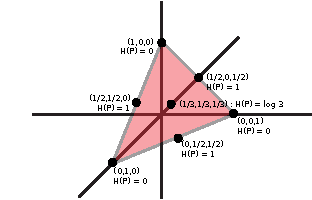
\includegraphics[width=\textwidth]{figures/prob-simplex-types3.pdf}
    \caption{Representação de alguns pontos e suas respectivas entropias.}
    \label{fig:prob-simplex-3t}
    \end{marginfigure}
  \end{example}



O Teorema da Codificação de Shannon é um dos resultados fundamentais da teoria
da informação, estabelecendo as condições sob as quais é possível representar
as informações produzidas por uma fonte i.i.d. com distribuição subjacente $Q$
sem que haja perdas, utilizando, para tanto uma taxa $R$.
O Teorema mostra que, se $R > H(Q)$, então existe um código de bloco universal
para representar a informação produzida pela fonte com probabilidade de erro
tendendo a zero à medida que o comprimento $n$ das sequências aumenta.
Por outro lado, se $R < H(Q)$, não é possível representar a informação da fonte
com probabilidade de erro evanescente.
No contexto do método de tipos, podemos formalizar esse teorema explorando a
estrutura das classes de tipo: como o número de tipos é polinomial em $n$,
enquanto o número de sequências é exponencial em $n$, e apenas os tipos próximos
de $Q$ ocorrem, para $n$ grande, é possível construir códigos universais que
codifiquem eficientemente as sequências produzidas pela fonte, usando aproximadamente 
$nH(Q)$ bits.

\begin{theorem}[Teorema da Codificação de Shannon]\label{thm:teocodshannontipos}
$\exists$ uma sequencia $(2^{nR},n)$ de códigos universais tais que $P_e^{(n)} \rightarrow 0$ para toda
distribuição $Q$ tal que $H(Q) < R$.
\end{theorem}
\begin{proof}
  Fixe $R > H(Q)$. Defina uma taxa para $n$ que é fixada a um fator polinomial:
  \begin{equation}
    R_n \triangleq R - \vert \mathcal{X} \vert \frac{\log (n+1)}{n} < R .
  \end{equation}
  Defina um conjunto de sequências que possuem entropia de tipo menor do que esta taxa:
  \begin{subequations}
    \begin{align}
       A_n &\triangleq \{ x_{1:n} \in \mathcal{X}^n : H(P_{x_{1:n}}) \leq R_n \} \\
           &= \left\{  \bigcup_{P \in \mathcal{P}_n} T(P) : H(P) \leq R_n \right\}
    \end{align}
  \end{subequations}
  A partir desta definição, teremos que
  \begin{subequations}
  \begin{align}
    \vert A_n \vert &= \sum_{P \in \mathcal{P}_n : H(P) \leq R_n} \vert T(P) \vert \leq \sum_{P \in \mathcal{P}_n : H(P) \leq R_n} 2^{nH(P)} \\
                    &\leq \sum_{P \in \mathcal{P}_n : H(P) \leq R_n} 2^{nR_n} \leq (n+1)^{\vert \mathcal{X} \vert} 2^{nR_n} \\
                    &= 2^{n \left( R_n + \vert \mathcal{X} \vert \frac{\log (n+1)}{n} \right)} = 2^{nR} .
  \end{align}
  \end{subequations}
  Como $\vert A_n \vert \leq 2^{nR}$, podemos indexar $A_n$ com $nR$ bits.

  O codificador será dado por
  \begin{equation}
  f_n (x_{1:n}) =
  \begin{cases}
  \text{índice de } x_{1:n} \text{ em } A_n ,     \quad \text{ se } x_{1:n} \in A_n \\
  0                                       ,       \quad \text{ caso contrário }.
  \end{cases}
  \end{equation}
  O codificador associará um índice a $x_{1:n}$ se $H(P_{x_{1:n}}) \leq  R_n$ (ou seja, $x_{1:n} \in A_n$);
  e não associará valor se $H(P_{x_{1:n}}) >  R_n$ (ou seja, $x_{1:n} \notin A_n$).
  Note que $f_n(\cdot)$ não depende da distribuição da fonte, apenas do ordenamento e de $\RealNumber^m$.
  Um erro ocorrerá se $x_{1:n} \notin A_n$.
  Os tipos podem ser representados por pontos em um Simplex Probabilístico, conforme ilustrado na \Cref{fig:type-simplex}.
\begin{marginfigure}%
  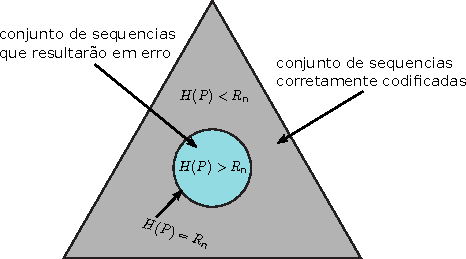
\includegraphics[width=\linewidth]{figures/type-simplex.pdf}
  \caption{Representação das sequências em um simplex probabilísticos. As sequências com $H(P_{x_{1:n}}) \leq  R_n$ não acarretarão em erro no processo de codificação.}
  \label{fig:type-simplex}
\end{marginfigure}
Um erro ocorre quando a sequência não está em $A_n$. Desta forma,
\begin{subequations}
  \begin{align}
  P_e^{(n)} = 1 - Q^n(A_n) &=& Q^n(A^c_n) = \sum_{P: H(P) > R_n} Q^n (T(P)) \\
        &\leq& \sum_{P: H(P) > R_n} \max_{P: H(P) > R_n} Q^n (T(P)) \\
        &\leq& (n+1)^{\vert \mathcal{X} \vert} \max_{P: H(P) > R_n} Q^n (T(P)) \\
        &\leq& (n+1)^{\vert \mathcal{X} \vert} \max_{P: H(P) > R_n} 2^{-n  D(P \mid\mid Q)} \\
        &=& (n+1)^{\vert \mathcal{X} \vert} 2^{-n [\min_{P: H(P) > R_n} D(P \mid\mid Q)]} \label{eq:dempeteoshan}
  \end{align}
\end{subequations}
onde utilizamos que $Q^n(T(P)) \leq 2^{-n D(P\mid \mid Q)}$.
Temos que $R_n$ forma uma sequência crescente com $n$, tal que $R_n < R$ para todo $n$ (veja a \Cref{fig:Rn-seq}).
Por hipótese, $H(Q) < R$. Eventualmente, para algum $n_0$, teremos que $\forall n > n_0$, $R_n > H(Q)$.
Na \Cref{eq:dempeteoshan}, escolhemos $P: H(P) > R_n$.
\begin{marginfigure}%
  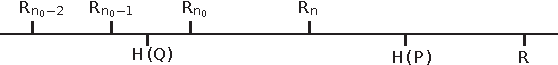
\includegraphics[width=\linewidth]{figures/Rn-seq.pdf}
  \caption{Sequência de taxas $R_n$.}
  \label{fig:Rn-seq}
\end{marginfigure}
Teremos então: $H(P) > R_n > H(Q)$, o que implica em $P \neq Q$.
Desta forma, teremos $D(P \mid\mid Q) > 0$, para $P$ que foi escolhido em \ref{eq:dempeteoshan}.
Teremos assim
\begin{equation}
  P_e^{(n)} \leq \underbrace{(n+1)^{\vert \mathcal{X} \vert}}_{\text{polinomial em } n} \underbrace{ 2^{-n [\min_{P: H(P) > R_n} D(P \mid\mid Q)]} }_{\text{exp. decrescente qnd } n \rightarrow \infty}
\end{equation}
Logo, $P_e^{(n)} \rightarrow 0$ quando $n \rightarrow \infty$.
\end{proof}
Por outro lado, se $R < H(Q)$ teremos $P_e^{(n)} \rightarrow 1$.
A entropia é então o limite de representação, ou compressão.
